\documentclass[12pt]{article}
\usepackage{graphicx}
\usepackage{hyperref}
\usepackage{listings}
\usepackage{graphicx}
\usepackage[T1]{fontenc}
\usepackage[polish]{babel}

\graphicspath{ {./images/} }

\lstset{mathescape}

\title{Raport projektu - \textit{Connect Four}}
\author{Mateusz Tkaczyk \\ Jakub Rudnik \\ Piotr Kurosad \\ Filip Łojek}
\date{8 marca 2024}

\begin{document}

\maketitle

\begin{abstract}
    Celem tego projektu było stworzenie modelu uczenia maszynowego zdolnego do skutecznego grania w grę \textit{Connect Four}. Aby osiągnąć ten cel, zaprojektowaliśmy i wdrożyliśmy dwa różne podejścia: regresyjne i klasyfikacyjne. Model regresyjny został zaprojektowany do przewidywania liczbowych wartości wyjściowych, reprezentujących ocenę danej pozycji. Natomiast model klasyfikacyjny miał na celu wytypowanie najlepszego ruchu spośród możliwych opcji, traktując to jako problem klasyfikacji.
\end{abstract}

\clearpage

\tableofcontents

\clearpage

\section{Wprowadzenie do projektu}

\subsection{Narzędzie i technologię}

W ramach naszego projektu korzystaliśmy z szeregu technologii i narzędzi, które umożliwiły efektywne stworzenie oraz wdrożenie modelu uczenia maszynowego do gry \textit{Connect Four}, jak również interaktywnego interfejsu użytkownika.

Cały projekt został napisany w języku \href{https://www.python.org/}{Python3}, korzystaliśmy z najnowszej na tamtą chwilę wersji \href{https://www.python.org/downloads/release/python-3119/}{3.11.9}. Do stworzenia modelu wykorzystaliśmy bibliotekę \href{https://www.tensorflow.org/}{TensorFlow} w wersji 2.16.1. Interfejs użytkownika został zaprogramowany dzięki użyciu biblioteki \href{https://www.pygame.org}{pygame} w wersji 2.5.2. Dodatkowo korzystaliśmy z dodatkowych narzędzi do pomniejszych zadań takich jak rozdzielenie zbiorów na treningowy i testowy za pomocą \href{https://scikit-learn.org/}{sklearn}, wczytanie danych dzięki \href{https://pandas.pydata.org/}{pandas}. Kluczową biblioteką, która była odpowiedzialna za operację na danych (oraz jest wewnętrznie wykorzystywana przez TensorFlow) jest \href{https://numpy.org/}{numpy}.

\subsection{Opis modeli}
Zadaniem algorytmu jest gra w klasyczną wersję \textit{Connect Four}. Użytkownik za pomocą interfejsu graficznego, będzie mógł grać przeciwko wybranemu algorytmowi. Do wyboru będą dwa modele:
\begin{itemize}
    \item klasyfikacyjny, w którym odpowiedzią modelu będzie ruch (dokładnie jego indeks od 0 do 6),
    \item regresywny, w którym odpowiedzią modelu będzie ewaluacja danej pozycji (dodatnie wartości świadczą o wygrywającej pozycji aktualnego gracza, 0 o remisie, a ujemne wartości o przegrywającej pozycji).
\end{itemize}

\noindent Danymi wejściowymi będzie plansza gry oraz informacja o tym, kto wykonuje następny ruch. Możliwe, że do modeli zostaną dostarczone dodatkowe informacje w zależności od potrzeb.


Dane treningowe oraz ewaluacyjne zostaną wygenerowane przez jeden z dostępnych silników do gry w \textit{Connect Four}.

\subsection{Zbieranie danych}
Dane zostały zebrane za pomocą optymalnego bota do \textit{Connect Four}. Ma on przeliczoną całą grę i mamy pewność, że dla każdej pozycji zwróci on nam dokładną ewaluację każdego ruchu. Ewaluuje on pozycje w następujący sposób (zakładając optymalny przebieg rozgrywki po każdym ruchu):

\begin{itemize}
    \item Jeśli po danym ruchu jesteśmy w stanie wygrać grę, to wynik tej ewaluacji jest dodatni.
    \item Jeśli po danym ruchu jesteśmy w stanie tylko przegrać, wynik ewaluacji jest ujemny.
    \item Jeśli dany ruch prowadzi do remisu, wynik ewaluacji to 0.
    \item Im wyższy
          wynik dodatni, tym szybciej po danym ruchu możemy wygrać, im bardziej ujemny wynik tym szybciej przegrywamy.
\end{itemize}

Dane zbieramy w następującym formacie:

\begin{lstlisting}
    $opis\_pozycji$, $ewaluacja_1$, $ewaluacja_2$, ..., $ewaluacja_7$
\end{lstlisting}


gdzie $opis\_pozycji$ jest wypisanymi jeden po drugim liczbami, oznaczającymi kolejne ruchy (indeksy kolumn, do których wrzucane były żetony) prowadzące do obecnej pozycji. $ewaluacja_i$ oznacza natomiast ewaluację ruchu do $i$-tej kolumny przy obecnej pozycji. Zdecydowaliśmy się dodatkowo na zebranie danych następującymi sposobami:

\begin{itemize}
    \item patrząc tylko na możliwe optymalne ruchy, budujemy drzewo optymalnych strategii,
    \item patrząc na wszystkie możliwe rozgrywki do danej głębokości, wygenerowaliśmy wszystkie rozgrywki do 8 ruchów od początku gry,
    \item generując zupełnie losowe rozgrywki,
    \item generując losowe rozgrywki, ale im lepszy ruch, tym większe prawdopodobieństwo mamy na jego wybranie.
\end{itemize}

Przy każdym z tych sposobów, każda wygenerowana pozycja ma przypisaną ewaluację każdego możliwego ruchu. Dzięki takiemu generowaniu danych, mamy nadzieję, że algorytm będzie w stanie poradzić sobie z graczem grającym dobre ruchy, ale jednocześnie powinien umieć wykorzystać błędy swojego przeciwnika.

\section{Opisy modeli}

\subsection{Model regresywny z planszą jako daną wejściową}

\subsubsection{Dane wejściowe}

Początkowa próba stworzenia modelu regresywnego opierała się na jednej danej wejściowej. Była to macierz o rozmiarach (6, 7, 2) składająca się z wartości logicznych. Reprezentowała ona jednoznacznie planszę do gry w \textit{Conenct Four}. Wymiary (6, 7) odpowiadają wymiarą planszy, a dodatkowy wymiar o wielkości 2, skorelowany jest z danym graczem. Jeżeli krążek pierwszego gracza znajduje się na planszy to w macierzy będzie symbolizowany jako wartość prawdziwa. Analogicznie dla drugiego gracza pamiętając, że żetony pierwszego gracza znajdują się w zerowej warstie, a drugiego w kolejnej.

\begin{figure}[!ht]
    \centering
    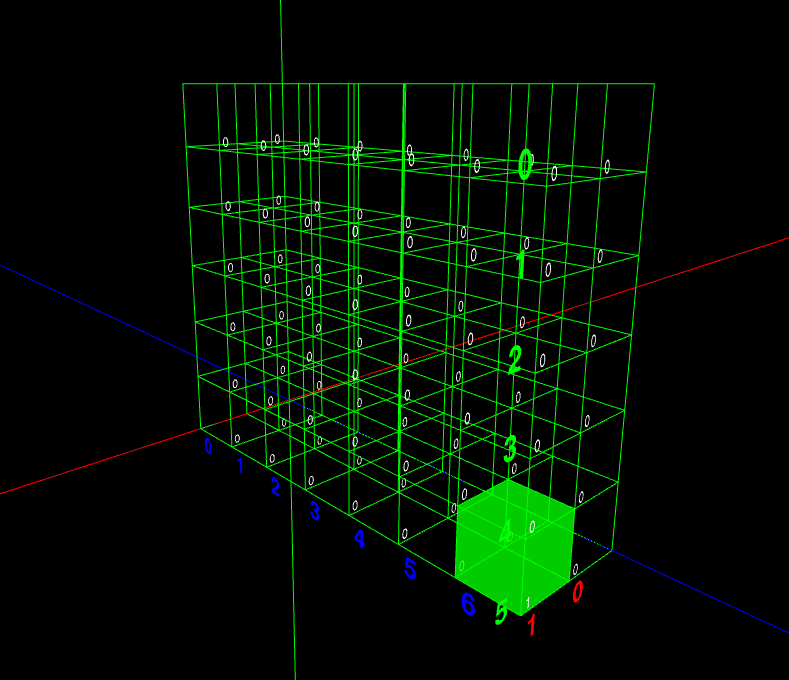
\includegraphics[scale=0.40]{board.png}
    \caption{Wizualna reprezentacja macierzy planszy, gdzie pierwszy gracz wykonał jedenyny ruch na 6 kolumnie.}
\end{figure}

W trakcie pracy nad modelem zdaliśmy sobie sprawę, że istotną informacją jaką należałoby dodać jest zmienna mówiąca, który gracz wykona ruch najbliższy ruch. Dla człowieka (lub innego rodzaju algorytmu) taka informacja może okazać się zbędna, ponieważ przy poprawnym tworzeniu planszy parzystość żetonów definiuje osobę, która wykonuje następny ruch. Jeżeli liczba jest nieparzysta pierwszy gracz musiał wykonać więcej ruchów, zatem następny powinien ruszyć się drugi gracz. W przeciwnym wypadku rusza się gracz pierwszy.

Zatem końcowo model jako dane wejściowe posiadał macierz o rozmiarach (6, 7, 2) jednoznacznie reprezentującą planszę oraz zmienną określającą gracza, który wykonuje ruch.

\subsubsection{Wielkość danych treningowych i testowych}

Podczas tworzenia modeli, do naszej dyspozycji było około 22 milionów plansz wraz z ich ewaluacjami. Jednak trenowanie na wszystkich dostępnych danych szybko okazał się nieefektywnym sposobem tworzenia modeli. Wielkość modelu, zmienną po której ocenaliśmy jego jakość i inne jego parametry zmienialiśmy w sposób dynamiczny analizując jakość uzyskanego algorytmu. Dzięki trenowaniu przy użyciu mniejszej ilości danych (około 100 tysięcy) byliśmy w stanie dostosowywać i zmieniać paramety modelu w znacznie szybszy sposób.

Do testowania modelu podeszliśmy w sposób bardziej kompleksowy. Zależało nam, aby wynik ewaluacji jakości modelu w jak najlepszy spsób odpowiadał jego rzeczywistej sile gry. Dlatego przy testowaniu każdego modelu używaliśmy wszystkich danych jakie mieliśmy do dyspozcji. Nawet jeżeli dany model był trenowany na mniejszej ilości danych, jego końcowa ewaluacja odbywała się na całym zbiorze.

\subsubsection{Rozmiar modelu w kontekście siły gry}

Pierwsze stworzone przez nas modele, miały dość mały rozmiar (około 40 tysięcy parametrów). W pewnym momencie, kolejne iteracje nie poprawiały jakości modelu. Kiedy pojawiał się taki problem, analizowaliśmy czy model nie potrzebuje innych danych wejściowych lub zmiany zbioru danych trenigowo-testowych. Następnie zwiększaliśmy liczbę jego parametrów. Taka zmiana poprawiała ewaluację danego modelu, nie tylko statystycznie, lecz również rosła realna siła gry algorytmu. Ostateczy model posiada około 84 milionów paramterów. Możliwym jest, że taka liczba parametrów przerasta liczbę stopni swobody gry w \textit{Connect Four}, ciężko jednak mówić o stopniach swobody, kiedy analizujemy teorie gier. Trudno jest stwierdzić, kiedy rozmiar modelu jest zbyt duży i zwiększanie go, nie przynosi realnych korzyści. Wówczas algorytm dopasowywuje się do danych jakimi go posiłkujemy, a nie do realnych zasad gry.

\subsubsection{Realna siła gry}

W trakcie rozwoju modelu opartego o planszę, jego jakość znacznie się zwiększała. Każda kolejna iteracja, czy to zmieniająca dane wejściowe, treningowe czy liczbę parametrów, poprawiała siłę analizy naszego algorytmu. Niestety te podejście spotkało się z pewnymi twardymi ograniczeniami, które okazały się dla nas przeszkodą w nalszym rozwijaniu dego podejścia. Nie byliśmy w stanie dalej polepszać jakości algorytmu mimo zastowania większej ilości danych, parametrów lub zmiany wewnętrzych ustawień (np. optymalizator, zmienna po której oceniamy jakość itd.). W końcowej wersji modelu, nie udało się nam uzyskać satysfakcjonującej siły gry. Algorytm potrafi wykonywać bardzo dobre ruchy, ale nie rozumie podstawowych zasad gry jak obronę kiedy przeciwnik ma 3 żetony w linii. Dochodzi do sytuacji, kiedy nasz model w momencie przegranej w jednym ruchu nie broni się, tylko wybiera inną kolumnę, skutującą natychmiastową przegraną. Nie tylko ma on trudności z człowiekiem, lecz również zbyt duży opór stanowi dla niego algorytm grający losowo. Zatem te podejście okazało się niepoprawne. Możliwe, że gdybyśmy zastosowali więcej danych wejściowych (np. mówiące o tym, czy przeciwnik ma wygraną w następnym ruchu), nasz algorytm uodpornił by się na ten problem. Postanowliśmy jednak spróbować rozwinąć nasze inne pomysły, które podchodzą do problemu w całkowicie inny sposób (np. bez podania planszy jako danej wejściowej).

\end{document}
